\documentclass[11pt,a4paper,fleqn,twoside]{article}
% Uncomment the following line to allow the usage of graphics (.png, .jpg)
\usepackage[pdftex]{graphicx}
\usepackage[a4paper,inner=2.2cm,outer=2.2cm,bottom=2.2cm,headheight=1cm]{geometry} % to change the page dimensions
% Comment the following line to NOT allow the usage of umlauts
\usepackage[utf8]{inputenc}
\usepackage[T1]{fontenc}
\usepackage{hyperref}

\usepackage{titling}
\renewcommand{\droptitle}{50pt}

\pretitle{%
  \begin{center}
  \LARGE
  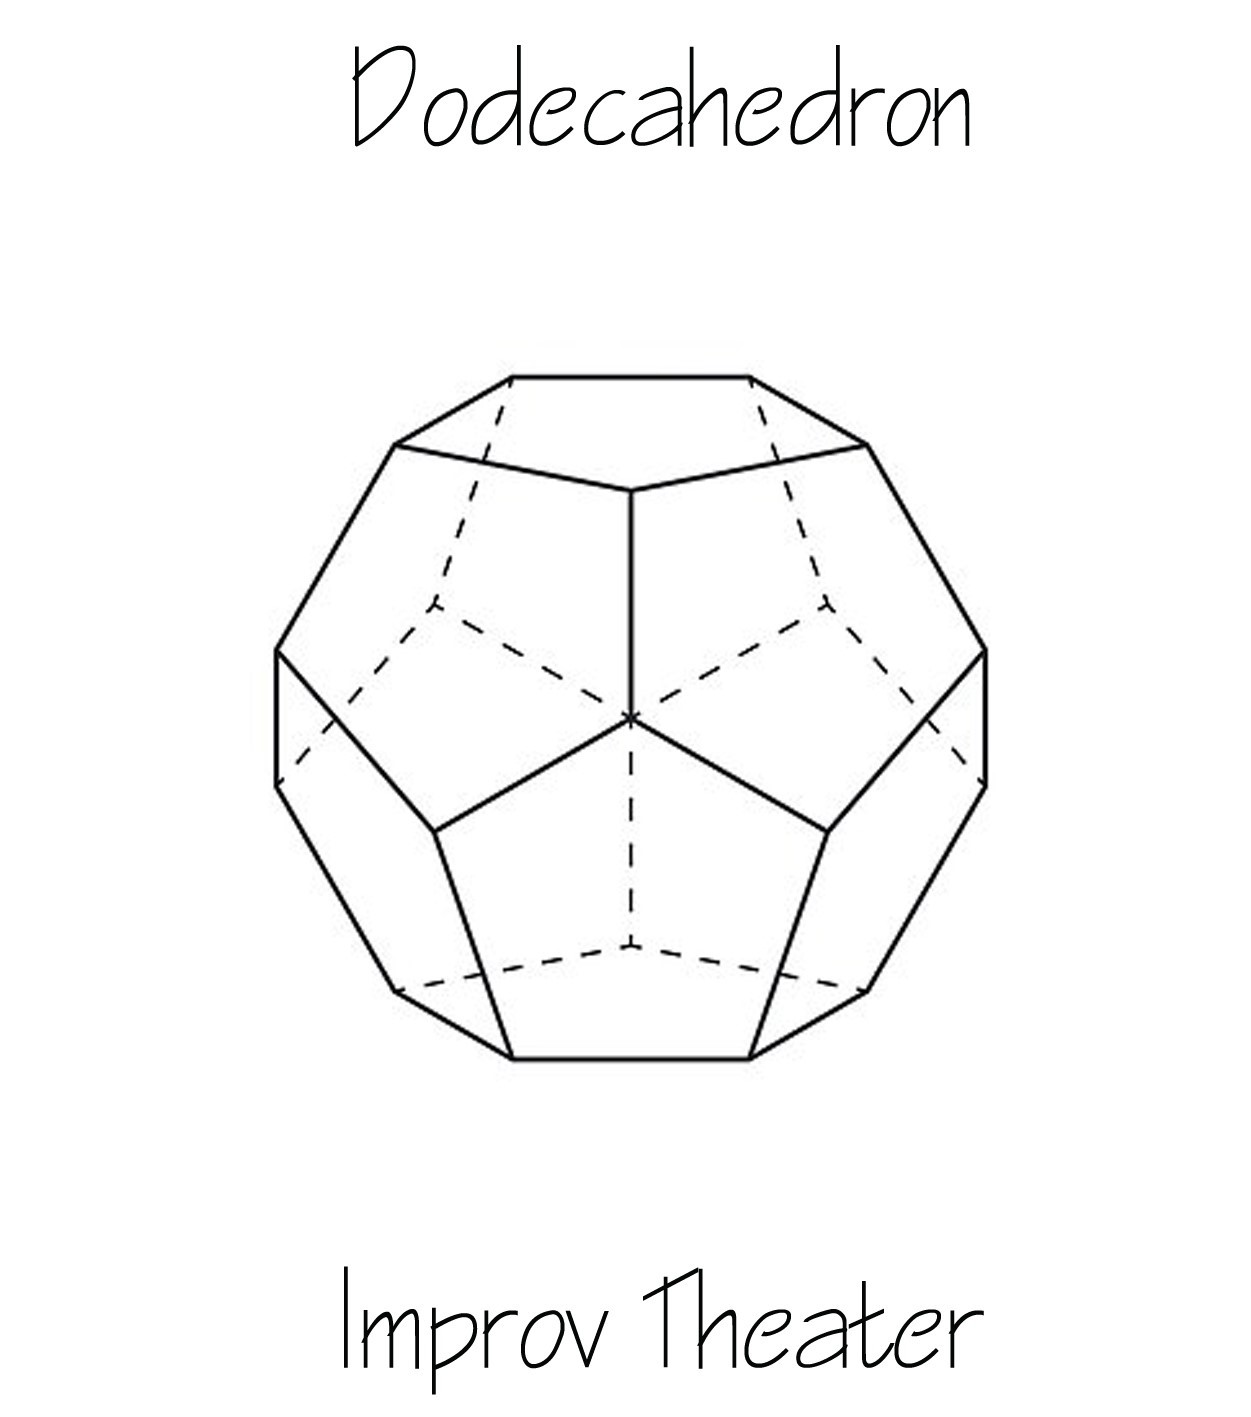
\includegraphics[width=0.6 \textwidth]{../../logo}\\[\bigskipamount]
}
\posttitle{\end{center}}
\title{Show proposal - March 2019}
\author{Dodecahedron Improv Group}

\begin{document}
\maketitle
\clearpage
\tableofcontents
%%%%%%%%%%%%%%%%%%%%%%%%%%%%
% Sections
\clearpage

\section{Introduction}

We are the Dodecahedron Improv Theater (DIT) group, a non-profit group of students and young professionals from different paths of life who gather on a weekly basis to learn and rehearse theater improvisation. Our group was brought to life in July 2017. We meet on weekly basis for rehearsals at ETH Zürich zentrum, usually on Wednesdays. One can find more updated information about us in our \href{https://www.facebook.com/dodecahedronimprovtheater/}{Facebook page}.

\subsection{Improvisational theater, Improv}

The improvisational theater or, also called ``Improv'' is just another form of theater. It just have the particularity that there is not predefined script of the story that it is going to be performed on the stage. Instead, it will be the actors of improvisers the ones in charge of creating it, on the go. In Improv the people on the stage are the actors, producers and directors of the ongoing plot, everything at the same time.

Their stories will usually be motivated by some external interaction. In occasions the audience will provide some aspect of the story to be told that will guide the improvisers, for example a relationship between characters, the place will the action will take place or a general idea that shall be translated into a plot. 

\section{March show proposal}

\subsection{Purpose}

We would want to use our sWith our upcoming show in March 

\subsection{Time allocation}

The idea would be to make the event in the second week of March, any day from March 4th to March 8th would be perfect. The starting time for the show would be 8pm and it would last between one hour and one hour and a half.

\subsection{Show description}

The type show that we will perform consists on the presentation of a series of plots which are developed around some predefined games. These games provide a particular challenge to the improviser that it's added on the top of this usual task to invent a story on the go. An overview of the games that are within the porfolio of the DIT are presented in Section \ref{sec:games}. For the show in March, the 	

\subsection{Logistics}

Our needs in terms of logistics are fairly minimal. We just require a small stage where up to four people could act without space restrictions. The audience shall be place in front of the space, preferably while sitting either on the floor or in chairs. We do not require any sound system. If possible, the lighting condition of the room shall be such that the stage is the most illuminated space in the room.

\section{Games} \label{sec:games}

The follonwing Sections described all the games are within the portfolio of the TIC.

\subsection{Deaths}
% The one in which you are given a why of dying. There are 3-4 people of the stage and they all have to die at the end of the story in the way they were told to.
This game consists

\subsection{The chairs}
% In this game, 3-4 people are sitting on chairs in the stage. On a signal provided by the moderator, they have to either stand up or remain sitted. Those of them who decide to stand up will need to create a story in a collaborative manner. On a second signal of the moderator, they need to sit down. 
This game consists

\end{document}